\documentclass[tikz]{standalone}
\usepackage{amssymb,amsmath,mathtools}

\usetikzlibrary{fit}
\usetikzlibrary{shapes,arrows}
\usetikzlibrary {shapes.misc} 
\usetikzlibrary{arrows.meta}
\usetikzlibrary{calc,positioning}
\usetikzlibrary{patterns,decorations.pathmorphing,decorations.markings}

\begin{document}

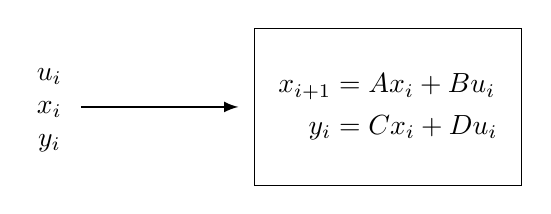
\begin{tikzpicture}[scale=2]
    \draw[thick, -latex] (0,3) -- (1,3);
    \node at (-0.2,3) {$\begin{matrix}
        u_i\\ 
        x_i\\
        y_i\\
      \end{matrix}$
      };
    \draw (1.1,2.5) rectangle (2.8,3.5);
    \node at (1.95,3) {
        $\begin{aligned}
            x_{i+1} &= Ax_i + Bu_i\\
            y_{i} &= Cx_i + Du_i				
        \end{aligned}$
    };
\end{tikzpicture}

\end{document}